\documentclass{tufte-handout}

\newcommand{\myroot}{../..}
\usepackage[handout]{\myroot/course}
\title{\usnaCourseNumber\ Task 3.1 -- Computer vision: acquiring images}
\author{\usnaInstructorShort}
\date{\printdate{\courseWeekTwo}}


\usepackage{tikz}
\tikzset{
block/.style={rectangle, minimum width=0.75in, minimum height=3em, text centered, align=center, draw=black, fill=blue!30},
arrow/.style={thick,<-,>=stealth},
noarrow/.style={thick}}

\begin{document}
\maketitle

%Goal
The syntax for acquiring images from a digital camera is dependent on the camera, drivers, and software selected for a given project. For this project, we need to interface a USB webcam with \Matlab\ to quickly acquire digital images.

\section{Prerequisites} 
This course requires use of \Matlab\ R2017b or later. \textbf{If your installation is not working, fix it right now\sidenote{Login to MathWorks (\url{https://www.mathworks.com/login}), download and install.}!} You will also need the \Matlab\ Image Processing Toolbox and the \Matlab\ Support Package for USB Webcams\sidenote{Open \Matlab\ as Administrator, run \lstinline{supportPackageInstaller} and install the necessary package.}. 
\marginnote{To install from MathWorks, you may need to login to your MathWorks account, which should be your USNA email address.}
 
For this set of exercises, you need the function \lstinline{initWebcam.m} in your current \Matlab\ directory or path\sidenote{Download from \url{https://github.com/kutzer/WRC_MATLABCameraSupport/archive/master.zip} or clone using Git, \lstinline{git clone https://github.com/kutzer/WRC_MATLABCameraSupport.git} into your \Matlab\ \usnaCourseNumber\ working directory}.
        
        
\section{Initializing the camera}
Camera selection (when applicable) and initialization is wrapped into a single \Matlab\ function\sidenote{If the camera has already been initialized, the function will provide an error message; you can either work with the existing handle or clear it using \lstinline{clear all}.}:
\begin{lstlisting}[style=usnaMatlab]
[cam,prv] = initWebcam; 
\end{lstlisting}
Calling \lstinline{initWebcam.m} with this syntax will do the following:
\begin{enumerate}
\item Initialize a webcam object with a handle contained in the variable \lstinline{cam} (short for webcam)
\item Initialize an image object with a handle contained in the variable \lstinline{prv} (short for preview)
\end{enumerate}

\subsection{Acquiring images}
Given a valid image object handle for your webcam preview (e.g. \lstinline{prv}), images can be quickly and easily acquired using either the \lstinline{get/set} syntax or the dot notation\sidenote{Both methods are acceptable, so pick whichever you like. Also note that the property name \lstinline{CData} is an abbreviation for ``Color Data''.}:
\begin{lstlisting}[style=usnaMatlab]
im = get(prv,'CData'); % this is equivalent to im = prv.CData
\end{lstlisting}
Or using dot notation:
\begin{lstlisting}[style=usnaMatlab]
im = prv.CData; % this is equivalent to im = get(prv,'CData')
\end{lstlisting}


\subsection{Observations}
In \Matlab, color images are represented as three-dimensional arrays. When using the RGB (red, green, blue) color space, the dimensions of the image will be $M\times N\times 3$, for example. In this context, $M$ represents the number of pixels vertically (i.e. the number of rows), and $N$ represents the number of pixels horizontally (i.e. the number of columns). The three layers or channels represent the pixel intensities in the red, green, and blue spectrum\sidenote{Thus, for the \usnaCourseNumber\ webcam, the images should be of shape \num{480x640x3}. Explore your image from the command line to verify its dimensions and content.}. For example, given an image named \lstinline{im}, the pixel intensity in the red spectrum can be isolated using:
\begin{lstlisting}[style=usnaMatlab]
im_Red = im(:,:,1); % gives red channel only, 480x640x1
\end{lstlisting}
the pixel intensity in the green spectrum can be isolated using:
\begin{lstlisting}[style=usnaMatlab]
im_Green = im(:,:,2); % gives green channel only, 480x640x1
\end{lstlisting}
and the pixel intensity in the blue spectrum can be isolated using:
\begin{lstlisting}[style=usnaMatlab]
im_Blue = im(:,:,3); % gives blue channel only, 480x640x1
\end{lstlisting}

\subsection{Plotting}
Generally, images can be plotted (displayed) in \Matlab\ using the function \lstinline{imshow.m}. For the purposes of code development in this course, it is always advisable to capture and use the \textbf{handles}\sidenote{Remember from EW200, \textbf{handles} are a way to grab a graphic object and do stuff to it by altering the handle \textbf{properties}.} of the graphics objects you create, e.g.
\begin{lstlisting}[style=usnaMatlab]
h = imshow(ax1,im); % h is a handle to the image
\end{lstlisting}
This will both speed up your code and eliminate inadvertent misplacement or duplication of graphics objects. 

\subsection{Parent-child relationships in \Matlab\ graphic objects}
In \Matlab, all graphics have an underlying dependency between parents and children. A basic example of \Matlab\ graphics dependency is given in \fref{fig:1}\sidenote{This forms a tree structure which can be traversed and operated on algorithmically and is sometimes of use when trying to group and move or operate on objects together.}.
\begin{figure*}
\begin{center}
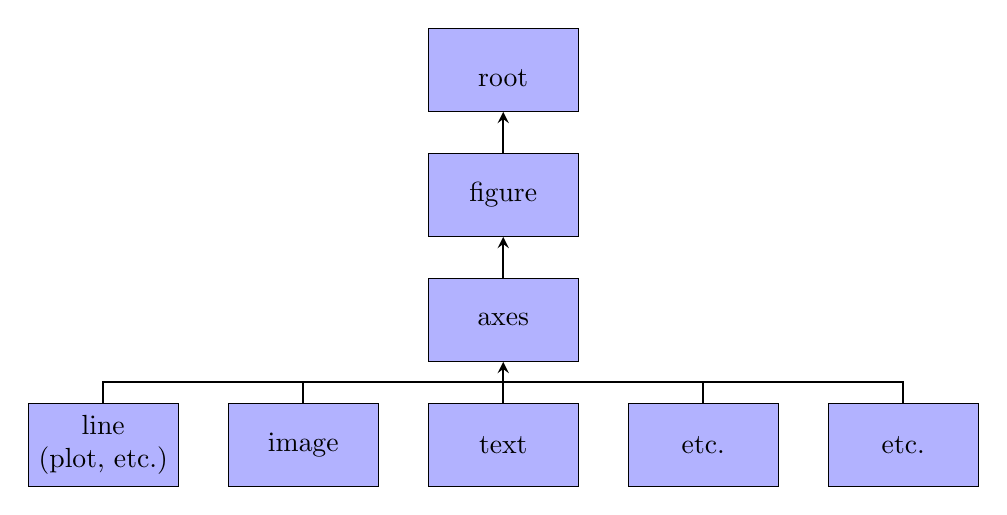
\begin{tikzpicture}
\node (root) [block] {\Matlab\\root};
\node (fig1) [block, below of=root, node distance=0.625in] {\lstinline{figure}};
\node (ax1) [block, below of=fig1, node distance=0.625in] {\lstinline{axes}};
\node (text) [block, below of=ax1, node distance=0.625in] {\lstinline{text}};
\coordinate [below of=ax1, node distance=0.3125in] (x); 
\node (image) [block, left of=text, node distance=1in] {\lstinline{image}};
\node (line) [block, left of=image, node distance=1in] {\lstinline{line}\\(\lstinline{plot}, etc.)};
\node (etc1) [block, right of=text, node distance=1in] {etc.};
\node (etc2) [block, right of=etc1, node distance=1in] {etc.};

\draw [arrow] (root) -- (fig1); 
\draw [arrow] (fig1) -- (ax1); 
\draw [arrow] (ax1) -- (text); 
\draw [noarrow] (image) |- (x); 
\draw [noarrow] (line) |- (x); 
\draw [noarrow] (etc1) |- (x); 
\draw [noarrow] (etc2) |- (x); 
\end{tikzpicture}

\end{center}
\caption{A basic example of \Matlab\ graphics dependency (tree). Arrows depict dependency and are shown pointing from child to parent.}
\label{fig:1}
\end{figure*}

A figure object (i.e. the window containing your plot) whose handle is contained in the variable \lstinline{figEXAMPLE} can be created using the following\sidenote{\lstinline{Parent 0} refers to the \Matlab\ root object}:
\begin{lstlisting}[style=usnaMatlab]
figEXAMPLE = figure('Parent',0);
\end{lstlisting}

An axes object that is contained in (i.e. a dependent or \textbf{child} of) the figure \lstinline{figExample} can be created using:
\begin{lstlisting}[style=usnaMatlab]
axsEXAMPLE = axes('Parent',figEXAMPLE);
\end{lstlisting}

Here, the handle of the newly created axes object is contained in the variable \lstinline{axsEXAMPLE}. 

This syntax is generally applicable when adding items to the axes, additional axes or panels to the figure, etc. As an example, an image contained in the variable \lstinline{im} can be created and added to the axes using:
\begin{lstlisting}[style=usnaMatlab]
imgEXAMPLE = imshow(im,'Parent',axsEXAMPLE);
\end{lstlisting}
where \lstinline{imgEXAMPLE} is now the handle of the newly created image object that we have added to axes \lstinline{axsEXAMPLE}. 

\section{Aside: working with \Matlab\ graphics object (handle class) properties}
Each graphics object in \Matlab\ can be updated by changing the properties associated with a given handle. The most common property that we change when plotting information is the \lstinline{NextPlot} property associated with axes objects. We commonly do so using the command:
\begin{lstlisting}[style=usnaMatlab]
hold(axsEXAMPLE,'on');
\end{lstlisting}
or, when ignoring graphics objects (which is rarely advisable but unfortunately all too convenient):
\begin{lstlisting}[style=usnaMatlab]
hold on
\end{lstlisting}
\lstinline{hold on} changes the \lstinline{NextPlot} property from the default value of \lstinline{'replace'} to the value \lstinline{'add'}. The result is that when calling subsequent \lstinline{plot} commands, the current axes object will add new graphics objects as additional children, rather than replacing the existing graphics objects. 

For uniformity, we recommend use of either the \lstinline{get/set} syntax or dot notation instead\sidenote{This also helps us explicitly keep track of which axes object we are working with.}:
\begin{lstlisting}[style=usnaMatlab]
set(axsEXAMPLE,'NextPlot','add'); % equivalent to hold on
\end{lstlisting}
or using the dot notation:
\begin{lstlisting}[style=usnaMatlab]
axsEXAMPLE.NextPlot = 'add'; % also equivalent to hold on
\end{lstlisting}

Some object properties, like \lstinline{NextPlot}, have a limited set of discrete values that are valid; while others have numeric or array values. To get a listing of all properties and current property values associated with a given object (e.g. \lstinline{axsEXAMPLE}) you can use:
\begin{lstlisting}[style=usnaMatlab]
get(axsEXAMPLE); % should print out the properties and their values
\end{lstlisting}
Similarly, to get a listing of the discrete options for all properties, you can use:
\begin{lstlisting}[style=usnaMatlab]
set(axsEXAMPLE); % should print out the options for all properties
\end{lstlisting}

\section{Bringing it all together}
Take the time to combine everything you have learned into a single \Matlab\ script to accomplish the following:
\begin{enumerate}
\item Initialize your camera and acquire an image\sidenote{You may wish to include a call to \lstinline{drawnow} immediately afterinitializing the camera to force it to update the image.}.
\item Create a figure named \lstinline{EW309 - Camera Overlay Test} (use the \lstinline{Name} property). You should see this name displayed in the title bar of the window. 
\item Create an axes in your figure and adjust the \lstinline{NextPlot} property.
\item Add your image to the axes.
\item Add a crosshair to the axes using two independent line objects (created using the \lstinline{line} or \lstinline{plot} functions).
\item Create an indefinite \lstinline{while} loop (using \lstinline{while true}):
\begin{enumerate}
\item Get the current image from the webcam preview object.
\item Update\sidenote{Rather than copy the same line and create a new image object, remember to \textbf{update} your existing image by updating the appropriate image property using its handle. This will help your loop run at a reasonable rate, which is important for control.} your image object color data with the new image (use the \lstinline{CData} property). 
\item Allow your plot to update\sidenote{Be sure you aren't just creating 100 new plots accidentally!} using the \lstinline{drawnow} command.
\end{enumerate}
\end{enumerate}
\end{document}
 


